\section{Method}
\label{sec:approach}

We first discuss the formulation of a scene graph in Sec.~\ref{sec:sg_formulation}. We then introduce how to generate a 3D outdoor scene conditioned on a scene graph in Sec.~\ref{sec:scene-graph-guided}. In Sec.~\ref{sec:interactive}, we describe how the proposed method facilitates the convenient creation of 3D scenes.

\subsection{Scene Graph Formulation}
\label{sec:sg_formulation}
%
Formally, a scene graph is characterized by its nodes and edges as \( \mathcal{G} = (\mathcal{V}, \mathcal{E}) \).
%
The set of nodes \( \mathcal{V} \) consists of two types (i.e., \( \mathcal{V} = \mathcal{V}_I \cup \mathcal{V}_R \)):
a) \textbf{Instance Nodes} (\( \mathcal{V}_I \)) that represent countable objects with standard labels defined in ~\cite{carlasc}, such as vehicles and pedestrians. 
%
Each node \( v_i \in \mathcal{V}_I \) is associated with a feature vector $[\mathbf{c}_i; \mathbf{p}_i]$, where \( \mathbf{c}_i \in \mathbb{R}^d \) denotes the node attributes with dimension $d$, and \( \mathbf{p}_i \in \mathbb{R}^2 \) represents a coordinate specifying its center position in the BEV map. 
%
b) \textbf{Scene Road Nodes} (\( \mathcal{V}_R \)) that define the structure of the road and other global background information of the scene in one node, i.e., $\mathcal{V}_R=\{v_r\}$. 
 %
We further construct the graph structure by defining two types of edges \( \mathcal{E} \) to capture essential relationships: a) \textbf{Physical Proximity}: For any two instance nodes \( v_i, v_j \in \mathcal{V}_I \), we define an edge \( e_{ij} \in \mathcal{E} \) if the Euclidean distance \( d_{ij} = \|\mathbf{p}_i - \mathbf{p}_j\| \)  is smaller than a threshold \( \delta_d \). b) \textbf{Road Connectivity}: For any instance node \( v_i \in \mathcal{V}_I \) and the singleton road node \( v_r \in \mathcal{V}_R \), an edge \( e_{ir} \in \mathcal{E} \) is created for the connects to the road structure. 

In practice, we use the simplified graph as control signals to ease user interaction, where each instance node contains only its semantic label $\mathbf{c}_i$ and an approximate 2D position $\mathbf{p}_i$ represented as a patch index. Also, the scene road node is represented by the road type.


\subsection{Scene-graph-guided Diffusion}
\label{sec:scene-graph-guided}


\begin{figure}[t]
    \centering
    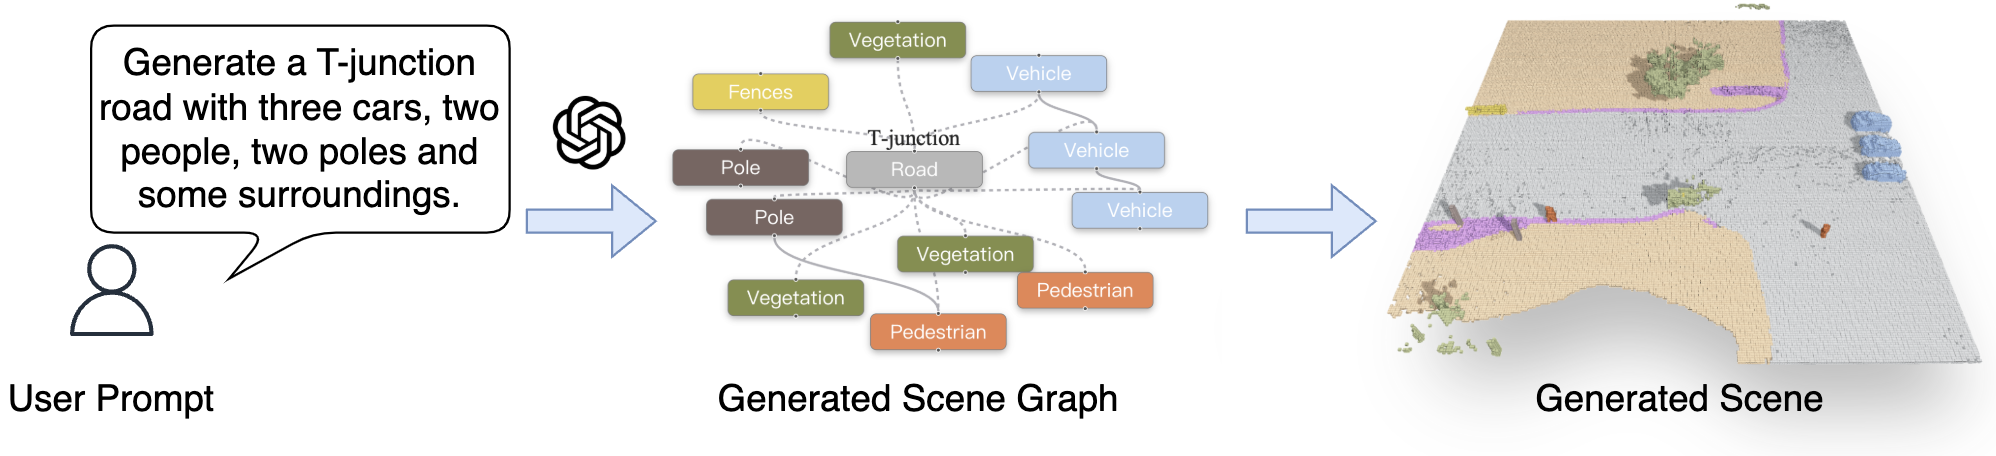
\includegraphics[width = 0.97\linewidth]
    {./fig/llm_generation_iccv.png}
    \vspace{-0.5em}
    \caption{\textbf{Scene Graph Generation.} LLMs convert the user’s prompt into a scene graph, which guides 3D scene generation.}
    \label{fig:prompt_generation}
    \vspace{-1em}
\end{figure}


Given a 2D scene graph, our method aims at generating a 3D semantic scene that aligns with the structure defined by the scene graph. In the following, we first convert the scene graph into a dense 2D embedding using a Graph Neural Network (GNN). Next, we synthesize a plausible 2D scene map by training a 2D diffusion model conditioned on the scene graph embedding. Finally, we use a conditional 3D diffusion model to generate the final 3D outdoor scene given the 2D scene map. 

\noindent \textbf{Scene Graph Neural Network}. 
\label{sec:gnn}
The scene Graph Neural Network (Fig.~\ref{fig:main_method}\textcolor{red}{(b)}) aims to generate node embeddings for scene graphs that capture both local structural and global context information. Particularly, we utilize  Graph Attention Network (GAT) \cite{gat} for GNN implementation.
%
Given a graph \( \mathcal{G} = (\mathcal{V}, \mathcal{E}) \),  with adjacency matrix \( \mathbf{A} \in \mathbb{R}^{|\mathcal{V}| \times |\mathcal{V}|} \) that encodes the connectivity between nodes, 
%
the node embeddings $\mathbf{h}_i$ are computed by a two-layer GAT for node \( v_i \) in the graph.  
%
To incorporate global context into the node embeddings, we concatenate each node’s embedding with a pooled global embedding \( \mathbf{h}_G \) as the final embedding, i.e.,
\small
\begin{equation}
   \mathbf{h}_i^{\text{CANE}} = \text{MLP}([\mathbf{h}_i;\mathbf{h}_G 
   ]), \mathbf{h}_G= \text{Pooling}(\{\mathbf{h}_i \mid v_i \in \mathcal{V}\}),
\end{equation}
\normalsize
where  \( [\cdot; \cdot] \) denotes concatenation,  \( \text{Pooling} (\cdot)\) is a graph global mean pooling operation~\cite{mesquita2020rethinking}, $\mathbf{h}_G \in \mathbb{R}^{64}$ and $\text{MLP}(\cdot)$ is a multi-layer perceptron. We name the output embedding $\mathbf{h}_i^{\text{CANE}}$ as Context-aware node embedding (CANE).


We train the GNN with two objectives: the auxiliary tasks (Fig.~\ref{fig:main_method}\textcolor{red}{(d)}) and the downstream task (Fig.~\ref{fig:main_method}\textcolor{red}{(e)}). 
%
For auxiliary tasks, we apply edge reconstruction loss as in Graph Auto-encoder (GAE)~\cite{gae} and node classification loss, given by
\small
\begin{equation}
\label{eq:a_loss}
     \mathcal{L}_a = \text{BCE}(\hat{\mathbf{A}}, \mathbf{A})+  \frac{1}{|\mathcal{V}|} \sum_{i=1}^{|\mathcal{V}|} \text{CE} (y_i, \hat{y}_i),
\end{equation}
\normalsize
where $\text{BCE}$ is binary cross-entropy, $\text{CE}$ is node-wise  cross-entropy loss, and,
% \begin{small}
\small
\begin{equation}
    \hat{\mathbf{A}} = \sigma(\mathbf{h}_G \mathbf{h}_G^\top), \hat{y}_i = \text{Softmax}(\text{MLP} (\mathbf{h}_i^\text{CANE})),
\end{equation} 
\normalsize
% \end{small}
for $\sigma(\cdot)$ being sigmoid function.
%
The first term of ~\eqref{eq:a_loss} is to reconstruct the global edge structure of the scene, specifically the adjacency matrix \( \mathbf{A} \). The second term of ~\eqref{eq:a_loss} is to classify each node \( v_i \) into the original category. 
%
The auxiliary tasks ensure that the network learns both structural relationships and node-specific features, effectively capturing both local and global information in the CANE. 

For downstream task,  embeddings \( \mathbf{h}_i^\text{CANE} \) are used as inputs to compute BEV Embedding Map (BEM, Fig.~\ref{fig:main_method}\textcolor{red}{(c)}) which serves as condition for the sequential diffusion model in the next phase of diffusion. 
%
These embeddings are passed to an \textbf{allocation module},  defined by
%\begin{small}
\small
\begin{equation}\label{eq:allocation}
    \mathbf{L} = \sum_{i=1}^{|\mathcal{V}|} \mathcal{M}(\hat{p}_i) \odot \mathbf{h}_i^\text{CANE},
\end{equation}
\normalsize
%\end{small}
where $\mathbf{L}\in \mathbb{R}^{H_b\times W_b\times C} $ is the output BEM with height $H_b$, width $W_b$, and channel dimension $C$. The binary map $ \mathcal{M}(\hat{p}_i)\in \{0,1\}^{H_b\times W_b}$ is expanded along the channel dimension to \( \mathbb{R}^{H_b \times W_b \times C} \) to enable element-wise multiplication with the node embedding \( \mathbf{h}_i^\text{CANE} \in \mathbb{R}^{C} \).  
%
In the implementation, we perform the inference by sampling position from an MLP-based localization head, i.e.,
%\begin{small}
\small
\begin{equation}
      \hat{p}_i \sim \text{GumbelSoftmax}_{\tau}(\text{Head}(\mathbf{h}_i^\text{CANE})),
\end{equation}
\normalsize
%\end{small}
where $\tau$ is the temperature for Gumbel softmax~\cite{jang2016categorical}. While in the training process of the diffusion model, we replace the $\hat{p}_i$ in ~\eqref{eq:allocation} by the ground truth position $p_i$. The localization head is trained after the diffusion model training. 
As a result, the allocation module effectively converts irregular and sparse graph representation into dense 2D map, i.e., BEM, which offers better compatibility with the subsequent 2D diffusion process.


\begin{figure*}[!t]
  \centering
  \includegraphics[width = 0.99\textwidth]
  {./fig/main_comparison_2_iccv.pdf}
  \vspace{-1em}
    \caption{\textbf{Controlling 3D Outdoor Scene Generation with Scene Graphs.} We compare baseline methods. Results show that our method generates scenes consistent with the provided scene graph, whereas the SG2Im and LLM approaches exhibit inconsistencies in object quantities and road types. 
    }
    \label{fig:main_comparison}
    \vspace{0em}
\end{figure*}

\noindent \textbf{2D Map Discrete Diffusion (Fig.~\ref{fig:main_method}\textcolor{red}{(f)}).} Given a scene graph, there may be multiple plausible 2D maps that align with its structure. To model this variability, we use a diffusion model that converts the sparse scene graph embedding into a dense 2D map representation.
%
Formally, the 2D Map Diffusion refines the sparse BEM $\mathbf{L}$ into a dense 2D map,  $\mathbf{X} \in \{0, 1\}^{H_b \times W_b \times c}$, where \( c \) is the semantic class number. We apply the standard discrete diffusion~\cite{austin2021structured} for 2D map generation.  
%
In the forward process, the 2D map \( \mathbf{X}_0 \) is gradually corrupted in \( T \) timesteps using a transition matrix \( \mathbf{Q}_t \), which adds noise as $\mathbf{X}_t = \mathbf{X}_{t-1} \mathbf{Q}_t$. 
%
This process can also be represented using a cumulative matrix \( \bar{\mathbf{Q}}_t \), allowing us to sample \( \mathbf{X}_t \) directly from the original map \( \mathbf{X}_0 \), 
% \begin{small}
\small
\begin{equation}
   q(\mathbf{X}_t \mid \mathbf{X}_0) = \operatorname{Cat}(\mathbf{X}_t; \mathbf{P} = \mathbf{X}_0 \bar{\mathbf{Q}}_t),
\end{equation}
\normalsize
% \end{small}
where \( \operatorname{Cat} \) represents a categorical distribution.

In the reverse diffusion stage, a model \( p_\theta \) learns to reverse the noise process, predicting the less-noised map \( \mathbf{X}_{t-1} \) from the noisy map \( \mathbf{X}_t \), using \( \mathbf{L} \) as guidance:
\small
\begin{equation}
%\begin{small}
   p_\theta(\mathbf{X}_{t-1} \mid \mathbf{X}_t, \mathbf{L}) = \mathbb{E}_{\tilde{p}_\theta(\tilde{\mathbf{X}}_0 \mid \mathbf{X}_t, \mathbf{L})} q(\mathbf{X}_{t-1} \mid \mathbf{X}_t, \tilde{\mathbf{X}}_0).
%\end{small}
\end{equation}
\normalsize
The model is trained by minimizing the KL divergence between the forward process and the learned reverse process. The loss function \( \mathcal{L}_\theta \) is defined as:
%\begin{small}
\small
\begin{align}\label{eq:diff_loss}
   \mathcal{L}_\theta =   & d_{\text{KL}}\left(q(\mathbf{X}_{t-1} \mid \mathbf{X}_t, \mathbf{X}_0) \| p_\theta(\mathbf{X}_{t-1} \mid \mathbf{X}_t, \mathbf{L})\right) \\\notag
   &+ \lambda d_{\text{KL}}\left(q(\mathbf{X}_0) \| \tilde{p}_\theta(\tilde{\mathbf{X}}_0 \mid \mathbf{X}_t, \mathbf{L})\right),
\end{align}
\normalsize
%\end{small}
where \( \lambda \) controls the weight of the auxiliary term for better reconstruction. During inference, we start from random noise and use the learned reverse diffusion to generate a dense 2D map \( \mathbf{X}_0 \), guided by the BEM \( \mathbf{L} \). This refined map provides a more complete spatial layout for further 3D scene generation. We train the GNN and the 2D map diffusion model using a loss 
% 
$\mathcal{L}_a+\mathcal{L}_{\theta}$. 
%

\noindent \textbf{3D Scene Discrete Diffusion (Fig.~\ref{fig:main_method}\textcolor{red}{(g)}).} We convert the generated 2D map into a dense 3D scene using a discrete diffusion process similar to the 2D Map Diffusion. The initial 2D map \( \mathbf{X}_0 \in \{0, 1\}^{H_d \times W_d \times c} \), generated from the previous diffusion step, is used as a condition to guide the generation of the 3D scene. We define the 3D scene as \( \mathbf{Z} \in \{0, 1\}^{H \times W \times D \times c} \), where \( H \), \( W \), and \( D \) are the dimensions of the 3D scenes and \( c \) represents semantic categories.

The 3D diffusion follows the same forward and reverse diffusion steps as in the 2D case but operates on the 3D scene grid. Specifically, a learnable model \( p_\phi \) predicts each denoised state \( \mathbf{Z}_{t-1} \) from \( \mathbf{Z}_t \), conditioned on the input 2D map \( \mathbf{X}_0 \), given by,
%\begin{small}
\small
\begin{equation}\label{eq:prob_3}
     p_\phi(\mathbf{Z}_{t-1} \mid \mathbf{Z}_t, \mathbf{X}_0)=\mathbb{E}_{\tilde{p}_\theta(\tilde{\mathbf{Z}}_0 \mid \mathbf{Z}_t, f(\mathbf{X}_0))} q(\mathbf{Z}_{t-1} \mid \mathbf{Z}_t, \tilde{\mathbf{Z}}_0),
\end{equation}
\normalsize
%\end{small}
where $f:\mathbb{R}^{H_d\times\ W_d\times c}\rightarrow \mathbb{R}^{H\times\ W \times c}$ is an up-scaling function. Furthermore, the training loss \( \mathcal{L}_\phi \) follows the same form as \eqref{eq:diff_loss}, given by,
%\begin{small}
\small
\begin{align}\label{eq:diff_loss2}
   \mathcal{L}_\phi =   & d_{\text{KL}}\left(q(\mathbf{Z}_{t-1} \mid \mathbf{Z}_t, \mathbf{Z}_0) \| p_\phi(\mathbf{Z}_{t-1} \mid \mathbf{Z}_t, \mathbf{X}_{0})\right) \\\notag
   &+ \lambda d_{\text{KL}}\left(q(\mathbf{Z}_0) \| \tilde{p}_\phi(\tilde{\mathbf{Z}}_0 \mid \mathbf{Z}_t, \mathbf{X}_{0})\right).
\end{align}
\normalsize
%\end{small}
During inference, the network generates the final 3D scene \( \mathbf{Z}_0 \) by starting from a noisy 3D state and applying the reverse diffusion process conditioned on \( \mathbf{X}_0 \). Specifically, each step of the reverse diffusion process is performed by sampling as ~\eqref{eq:prob_3}.
%
This produces a fully detailed 3D scene aligned with the spatial layout of the 2D map.


\begin{table*}[!t]
\centering
\caption{\textbf{Comparison of Different Conditioning Methods on 3D Outdoor Scene Generation.} Uncon-Gen, SG2Im, and LLM represent Unconditional Generation, Scene Graph to Image, and Large Language Model, while M-Pole, M-Pede, and M-Vech represent the MAE calculated individually for \textit{Pole}, \textit{Pedestrian}, and \textit{Vehicle} categories. In the Scene Quality Evaluation, higher mIoU and MA scores indicate better semantic consistency, while a lower F3D score~\cite{pdd} signifies closer feature alignment with the original dataset. In the Control Capacity Evaluation, a lower MAE reflects a smaller discrepancy between the generated scene and the object quantities defined in the scene graph for conditioning. A higher Jaccard Index indicates greater alignment in the object categories between the generated scenes and the specified scene graph.}
\vspace{-0.5em}
\resizebox{1\textwidth}{!}{
\begin{tabular}{cc|ccc|ccccc}
\toprule
\multirow{2}{*}{\textbf{Method}} & \multirow{2}{*}{\textbf{Condition}} & \multicolumn{3}{c|}{\textbf{Scene Quality}}               & \multicolumn{5}{c}{\textbf{Control Capacity}}                                                                     \\
                        &                            & mIoU           & MA             & \multicolumn{1}{c|}{F3D (\(\downarrow\))}               & MAE (\(\downarrow\)) & Jaccard       & M-Pole (\(\downarrow\)) & M-Pede (\(\downarrow\)) & M-Vech (\(\downarrow\)) \\ \midrule \midrule
Uncon-Gen~\cite{pdd}               & -                          & 68.21          & \textbf{85.69} & \multicolumn{1}{c|}{\textbf{0.338}}          & 2.07                 & 0.68          & 4.78                    & 4.71                    & 3.59                    \\ \midrule
SG2Im~\cite{johnson2018image}               & Scene Graph              & 65.43          & 81.72          & \multicolumn{1}{c|}{0.486} & 0.97                 & 0.81          & 2.25                    & 2.79                    & 2.64                    \\
LLM~\cite{ye2024language, zhao2023graphtext}               & Text-Embedding              & 68.19          & 85.62          & \multicolumn{1}{c|}{0.386} & 1.44                 & 0.70          & 3.41                    & 3.57                    & 3.51                    \\
\textbf{Ours}              & Scene Graph            & \textbf{68.69} & 85.01          & \multicolumn{1}{c|}{0.393}          & \textbf{0.63}        & \textbf{0.93} & \textbf{1.39}           & \textbf{1.81}           & \textbf{1.35}           \\ \bottomrule
\end{tabular}}
\label{tab:main_results}
 \vspace{0em}
\end{table*}




\begin{figure*}[t]
  \centering
  \includegraphics[width = 1\textwidth]
  {./fig/diversity_2.pdf}
  \vspace{-2em}
    \caption{\textbf{Diversity in Scene Generation.} Comparison of three scenes generated by our method under the same scene graph. This demonstrates our method’s ability to produce varied yet consistent scenes based on identical input.
    }
    \label{fig:diversity}
    % \vspace{-1.5em}
\end{figure*}


\subsection{Interactive System}
\label{sec:interactive}
%
We develop an interactive control system (Fig.~\ref{fig:main_method}\textcolor{red}{(a)}) that prioritizes user-directed scene graph manipulation. The core component is a graphical interface where users can precisely construct and modify scene graphs through intuitive operations such as node addition, deletion, and position adjustment. This direct manipulation ensures fine-grained control over the scene generation. Additionally, users can provide text prompts, which are processed by large language models to generate corresponding scene graphs (Fig.~\ref{fig:prompt_generation}). These scene graphs are then used as input to our method to generate the final 3D scenes. Details on the design of system-level prompts can be found in the supplementary materials.
%

